% Options for packages loaded elsewhere
% Options for packages loaded elsewhere
\PassOptionsToPackage{unicode}{hyperref}
\PassOptionsToPackage{hyphens}{url}
\PassOptionsToPackage{dvipsnames,svgnames,x11names}{xcolor}
%
\documentclass[
  10pt,
]{article}
\usepackage{xcolor}
\usepackage[margin=2cm]{geometry}
\usepackage{amsmath,amssymb}
\setcounter{secnumdepth}{5}
\usepackage{iftex}
\ifPDFTeX
  \usepackage[T1]{fontenc}
  \usepackage[utf8]{inputenc}
  \usepackage{textcomp} % provide euro and other symbols
\else % if luatex or xetex
  \usepackage{unicode-math} % this also loads fontspec
  \defaultfontfeatures{Scale=MatchLowercase}
  \defaultfontfeatures[\rmfamily]{Ligatures=TeX,Scale=1}
\fi
\usepackage{lmodern}
\ifPDFTeX\else
  % xetex/luatex font selection
\fi
% Use upquote if available, for straight quotes in verbatim environments
\IfFileExists{upquote.sty}{\usepackage{upquote}}{}
\IfFileExists{microtype.sty}{% use microtype if available
  \usepackage[]{microtype}
  \UseMicrotypeSet[protrusion]{basicmath} % disable protrusion for tt fonts
}{}
\makeatletter
\@ifundefined{KOMAClassName}{% if non-KOMA class
  \IfFileExists{parskip.sty}{%
    \usepackage{parskip}
  }{% else
    \setlength{\parindent}{0pt}
    \setlength{\parskip}{6pt plus 2pt minus 1pt}}
}{% if KOMA class
  \KOMAoptions{parskip=half}}
\makeatother
% Make \paragraph and \subparagraph free-standing
\makeatletter
\ifx\paragraph\undefined\else
  \let\oldparagraph\paragraph
  \renewcommand{\paragraph}{
    \@ifstar
      \xxxParagraphStar
      \xxxParagraphNoStar
  }
  \newcommand{\xxxParagraphStar}[1]{\oldparagraph*{#1}\mbox{}}
  \newcommand{\xxxParagraphNoStar}[1]{\oldparagraph{#1}\mbox{}}
\fi
\ifx\subparagraph\undefined\else
  \let\oldsubparagraph\subparagraph
  \renewcommand{\subparagraph}{
    \@ifstar
      \xxxSubParagraphStar
      \xxxSubParagraphNoStar
  }
  \newcommand{\xxxSubParagraphStar}[1]{\oldsubparagraph*{#1}\mbox{}}
  \newcommand{\xxxSubParagraphNoStar}[1]{\oldsubparagraph{#1}\mbox{}}
\fi
\makeatother

\usepackage{color}
\usepackage{fancyvrb}
\newcommand{\VerbBar}{|}
\newcommand{\VERB}{\Verb[commandchars=\\\{\}]}
\DefineVerbatimEnvironment{Highlighting}{Verbatim}{commandchars=\\\{\}}
% Add ',fontsize=\small' for more characters per line
\usepackage{framed}
\definecolor{shadecolor}{RGB}{241,243,245}
\newenvironment{Shaded}{\begin{snugshade}}{\end{snugshade}}
\newcommand{\AlertTok}[1]{\textcolor[rgb]{0.68,0.00,0.00}{#1}}
\newcommand{\AnnotationTok}[1]{\textcolor[rgb]{0.37,0.37,0.37}{#1}}
\newcommand{\AttributeTok}[1]{\textcolor[rgb]{0.40,0.45,0.13}{#1}}
\newcommand{\BaseNTok}[1]{\textcolor[rgb]{0.68,0.00,0.00}{#1}}
\newcommand{\BuiltInTok}[1]{\textcolor[rgb]{0.00,0.23,0.31}{#1}}
\newcommand{\CharTok}[1]{\textcolor[rgb]{0.13,0.47,0.30}{#1}}
\newcommand{\CommentTok}[1]{\textcolor[rgb]{0.37,0.37,0.37}{#1}}
\newcommand{\CommentVarTok}[1]{\textcolor[rgb]{0.37,0.37,0.37}{\textit{#1}}}
\newcommand{\ConstantTok}[1]{\textcolor[rgb]{0.56,0.35,0.01}{#1}}
\newcommand{\ControlFlowTok}[1]{\textcolor[rgb]{0.00,0.23,0.31}{\textbf{#1}}}
\newcommand{\DataTypeTok}[1]{\textcolor[rgb]{0.68,0.00,0.00}{#1}}
\newcommand{\DecValTok}[1]{\textcolor[rgb]{0.68,0.00,0.00}{#1}}
\newcommand{\DocumentationTok}[1]{\textcolor[rgb]{0.37,0.37,0.37}{\textit{#1}}}
\newcommand{\ErrorTok}[1]{\textcolor[rgb]{0.68,0.00,0.00}{#1}}
\newcommand{\ExtensionTok}[1]{\textcolor[rgb]{0.00,0.23,0.31}{#1}}
\newcommand{\FloatTok}[1]{\textcolor[rgb]{0.68,0.00,0.00}{#1}}
\newcommand{\FunctionTok}[1]{\textcolor[rgb]{0.28,0.35,0.67}{#1}}
\newcommand{\ImportTok}[1]{\textcolor[rgb]{0.00,0.46,0.62}{#1}}
\newcommand{\InformationTok}[1]{\textcolor[rgb]{0.37,0.37,0.37}{#1}}
\newcommand{\KeywordTok}[1]{\textcolor[rgb]{0.00,0.23,0.31}{\textbf{#1}}}
\newcommand{\NormalTok}[1]{\textcolor[rgb]{0.00,0.23,0.31}{#1}}
\newcommand{\OperatorTok}[1]{\textcolor[rgb]{0.37,0.37,0.37}{#1}}
\newcommand{\OtherTok}[1]{\textcolor[rgb]{0.00,0.23,0.31}{#1}}
\newcommand{\PreprocessorTok}[1]{\textcolor[rgb]{0.68,0.00,0.00}{#1}}
\newcommand{\RegionMarkerTok}[1]{\textcolor[rgb]{0.00,0.23,0.31}{#1}}
\newcommand{\SpecialCharTok}[1]{\textcolor[rgb]{0.37,0.37,0.37}{#1}}
\newcommand{\SpecialStringTok}[1]{\textcolor[rgb]{0.13,0.47,0.30}{#1}}
\newcommand{\StringTok}[1]{\textcolor[rgb]{0.13,0.47,0.30}{#1}}
\newcommand{\VariableTok}[1]{\textcolor[rgb]{0.07,0.07,0.07}{#1}}
\newcommand{\VerbatimStringTok}[1]{\textcolor[rgb]{0.13,0.47,0.30}{#1}}
\newcommand{\WarningTok}[1]{\textcolor[rgb]{0.37,0.37,0.37}{\textit{#1}}}

\usepackage{longtable,booktabs,array}
\newcounter{none} % for unnumbered tables
\usepackage{calc} % for calculating minipage widths
% Correct order of tables after \paragraph or \subparagraph
\usepackage{etoolbox}
\makeatletter
\patchcmd\longtable{\par}{\if@noskipsec\mbox{}\fi\par}{}{}
\makeatother
% Allow footnotes in longtable head/foot
\IfFileExists{footnotehyper.sty}{\usepackage{footnotehyper}}{\usepackage{footnote}}
\makesavenoteenv{longtable}
\usepackage{graphicx}
\makeatletter
\newsavebox\pandoc@box
\newcommand*\pandocbounded[1]{% scales image to fit in text height/width
  \sbox\pandoc@box{#1}%
  \Gscale@div\@tempa{\textheight}{\dimexpr\ht\pandoc@box+\dp\pandoc@box\relax}%
  \Gscale@div\@tempb{\linewidth}{\wd\pandoc@box}%
  \ifdim\@tempb\p@<\@tempa\p@\let\@tempa\@tempb\fi% select the smaller of both
  \ifdim\@tempa\p@<\p@\scalebox{\@tempa}{\usebox\pandoc@box}%
  \else\usebox{\pandoc@box}%
  \fi%
}
% Set default figure placement to htbp
\def\fps@figure{htbp}
\makeatother





\setlength{\emergencystretch}{3em} % prevent overfull lines

\providecommand{\tightlist}{%
  \setlength{\itemsep}{0pt}\setlength{\parskip}{0pt}}



 


\usepackage{graphicx}
\usepackage{amsmath}
\usepackage{booktabs}
\usepackage{float}
\usepackage{caption}
\usepackage{setspace}
\usepackage{fancyhdr}
\captionsetup{font=small}
\singlespacing
\pagestyle{fancy}
\fancyhf{}
\fancyfoot[C]{\thepage}
\makeatletter
\@ifpackageloaded{caption}{}{\usepackage{caption}}
\AtBeginDocument{%
\ifdefined\contentsname
  \renewcommand*\contentsname{Table of contents}
\else
  \newcommand\contentsname{Table of contents}
\fi
\ifdefined\listfigurename
  \renewcommand*\listfigurename{List of Figures}
\else
  \newcommand\listfigurename{List of Figures}
\fi
\ifdefined\listtablename
  \renewcommand*\listtablename{List of Tables}
\else
  \newcommand\listtablename{List of Tables}
\fi
\ifdefined\figurename
  \renewcommand*\figurename{Figure}
\else
  \newcommand\figurename{Figure}
\fi
\ifdefined\tablename
  \renewcommand*\tablename{Table}
\else
  \newcommand\tablename{Table}
\fi
}
\@ifpackageloaded{float}{}{\usepackage{float}}
\floatstyle{ruled}
\@ifundefined{c@chapter}{\newfloat{codelisting}{h}{lop}}{\newfloat{codelisting}{h}{lop}[chapter]}
\floatname{codelisting}{Listing}
\newcommand*\listoflistings{\listof{codelisting}{List of Listings}}
\makeatother
\makeatletter
\makeatother
\makeatletter
\@ifpackageloaded{caption}{}{\usepackage{caption}}
\@ifpackageloaded{subcaption}{}{\usepackage{subcaption}}
\makeatother
\usepackage{bookmark}
\IfFileExists{xurl.sty}{\usepackage{xurl}}{} % add URL line breaks if available
\urlstyle{same}
\hypersetup{
  pdftitle={Práctica perfiles usando una MLP},
  pdfauthor={Ismael Maximiliano De Los Santos Huesca},
  colorlinks=true,
  linkcolor={blue},
  filecolor={Maroon},
  citecolor={Blue},
  urlcolor={Blue},
  pdfcreator={LaTeX via pandoc}}


\title{Práctica perfiles usando una MLP}
\author{Ismael Maximiliano De Los Santos Huesca}
\date{2026-11-13}
\begin{document}
\maketitle

\begin{titlepage}

    % Logos alineados izquierda y derecha
    \begin{minipage}{0.45\textwidth}
        \raggedright
        
\includegraphics[width=7cm]{Logo_UNAM.png}
    \end{minipage}
    \hfill
    \begin{minipage}{0.45\textwidth}
        \raggedleft
        
\includegraphics[width=3.4cm]{Logo_LCG.png}
    \end{minipage}

    \centering
    \vspace*{2cm}

    {\Huge\bfseries Práctica predicción perfiles MLP \par}
    \vspace{2cm}
    
    {\Large Data Science \par}
    \vspace{1cm}
    
    {\Large De Los Santos Huesca Ismael Maximiliano \par}
    \vspace{1cm}

    {\Large Dr. Carlos Mendez\par}
    \vspace{1cm}
    
    {\Large Fecha: 12 Noviembre 2026 \par}
    
    \vfill

\end{titlepage}


\section{Carga de Datos y preprocesamiento\#\textbar{}
python.reticulate:
false}\label{carga-de-datos-y-preprocesamiento-python.reticulate-false}

\subsection{Lectura de datos y exploración
inicial}\label{lectura-de-datos-y-exploraciuxf3n-inicial}

\begin{Shaded}
\begin{Highlighting}[]
\CommentTok{\# leer los data sets}
\NormalTok{df\_data }\OperatorTok{=}\NormalTok{ pd.read\_csv(}
    \StringTok{"/mnt/c/Users/vrahu/Documents/Ismadlsh/CCG/2026{-}S5/Data\_Science/data/perfiles.csv"}\NormalTok{,}
\NormalTok{    index\_col}\OperatorTok{=}\DecValTok{0}\NormalTok{,}
\NormalTok{).rename\_axis(}\VariableTok{None}\NormalTok{)}

\NormalTok{df\_cathegories }\OperatorTok{=}\NormalTok{ pd.read\_csv(}
    \StringTok{"/mnt/c/Users/vrahu/Documents/Ismadlsh/CCG/2026{-}S5/Data\_Science/data/categorias\_perfiles.csv"}\NormalTok{,}
\NormalTok{    index\_col}\OperatorTok{=}\DecValTok{0}\NormalTok{,}
\NormalTok{).rename\_axis(}\VariableTok{None}\NormalTok{)}

\CommentTok{\# unir los data sets por el index}
\NormalTok{df\_data }\OperatorTok{=}\NormalTok{ pd.merge(df\_data, df\_cathegories, left\_index}\OperatorTok{=}\VariableTok{True}\NormalTok{, right\_index}\OperatorTok{=}\VariableTok{True}\NormalTok{)}
\BuiltInTok{print}\NormalTok{(}\StringTok{"Dimensionalidad de datos:"}\NormalTok{, df\_data.shape)}
\NormalTok{class\_u }\OperatorTok{=}\NormalTok{ df\_cathegories.Categoria.unique()}
\BuiltInTok{print}\NormalTok{(}\StringTok{"Categorías verdaderas únicas:"}\NormalTok{, class\_u)}
\NormalTok{df\_data.head()}
\end{Highlighting}
\end{Shaded}

Se observo que el dataset contiene 20531 genes y 5 categorías de
perfiles de expresión. Por ende los perfiles de expresión se tomaron
como variables yua numericas mientras que las categorías el cual es la
variable a predecir se deben transformar conserbando la información.

\subsubsection{Categorias a numerico}\label{categorias-a-numerico}

\begin{Shaded}
\begin{Highlighting}[]
\NormalTok{cat\_ids }\OperatorTok{=}\NormalTok{ \{cat\_u: i }\ControlFlowTok{for}\NormalTok{ i, cat\_u }\KeywordTok{in} \BuiltInTok{enumerate}\NormalTok{(class\_u)\}}

\NormalTok{ids\_cat }\OperatorTok{=}\NormalTok{ \{cat[}\DecValTok{1}\NormalTok{]: cat[}\DecValTok{0}\NormalTok{] }\ControlFlowTok{for}\NormalTok{ cat }\KeywordTok{in}\NormalTok{ cat\_ids.items()\}}
\end{Highlighting}
\end{Shaded}

\subsection{Split de los datos}\label{split-de-los-datos}

Consiguientemente se dividieron los datos en un 80\% para entrenamiento
y un 20\% para prueba, estratificando por la variable de categoría para
mantener la proporción de clases en ambos conjuntos.

\begin{Shaded}
\begin{Highlighting}[]

\NormalTok{df\_train, df\_test }\OperatorTok{=}\NormalTok{ train\_test\_split(df\_data, }
\NormalTok{    test\_size}\OperatorTok{=}\FloatTok{0.2}\NormalTok{, random\_state}\OperatorTok{=}\DecValTok{42}\NormalTok{, stratify}\OperatorTok{=}\NormalTok{df\_data.Categoria)}

\BuiltInTok{print}\NormalTok{(}\StringTok{"Dimensionalidad de datos de entrenamiento:"}\NormalTok{, df\_train.shape)}
\BuiltInTok{print}\NormalTok{(}\StringTok{"Dimensionalidad de datos de prueba:"}\NormalTok{, df\_test.shape)}
\end{Highlighting}
\end{Shaded}

\section{Modelado}\label{modelado}

\subsection{Creación data set}\label{creaciuxf3n-data-set}

\begin{Shaded}
\begin{Highlighting}[]
\CommentTok{\# Definición de la clase a partir del módulo Dataset de PyTorch}
\KeywordTok{class}\NormalTok{ PerfilesDataset(Dataset):}
    \KeywordTok{def} \FunctionTok{\_\_init\_\_}\NormalTok{(}\VariableTok{self}\NormalTok{, dataframe):}
        \CommentTok{\# Definimos dos atributos de la clase:}
        \CommentTok{\# {-} El DataFrame de donde crearemos el DataSet}
        \VariableTok{self}\NormalTok{.data }\OperatorTok{=}\NormalTok{ dataframe}
        \CommentTok{\# {-} El número de registros del DataSet}
        \VariableTok{self}\NormalTok{.}\BuiltInTok{len} \OperatorTok{=} \BuiltInTok{len}\NormalTok{(dataframe)}

    \KeywordTok{def} \FunctionTok{\_\_getitem\_\_}\NormalTok{(}\VariableTok{self}\NormalTok{, index):}
        \CommentTok{\# Guardamos en una variable el perfil de expresión separado de la categoría}
        \CommentTok{\# El procedimiento "drop" con "axis = 1" elimina una columna del DataFrame}
        \CommentTok{\# El procedimiento "iloc" localiza y entrega el registro "index" del DataFrame}
\NormalTok{        perfil\_de\_expresion }\OperatorTok{=} \VariableTok{self}\NormalTok{.data.drop([}\StringTok{"Categoria"}\NormalTok{], axis}\OperatorTok{=}\DecValTok{1}\NormalTok{).iloc[index].values}
        \CommentTok{\# Guardamos en una variable la categoría separada del perfil de expresión}
\NormalTok{        categoria }\OperatorTok{=} \VariableTok{self}\NormalTok{.data.Categoria.iloc[index]}

        \CommentTok{\# Convertimos la categoría en id con nuestro diccionario}
\NormalTok{        encoded\_categoria }\OperatorTok{=}\NormalTok{ cat\_ids[categoria]}

        \CommentTok{\# Convertimos variables con el perfil y la categoría en tensores de PyTorch}
\NormalTok{        tensor\_perfil\_de\_expresion }\OperatorTok{=}\NormalTok{ torch.as\_tensor(perfil\_de\_expresion)}
\NormalTok{        tensor\_categoria }\OperatorTok{=}\NormalTok{ torch.as\_tensor(encoded\_categoria)}
        \ControlFlowTok{return}\NormalTok{ tensor\_perfil\_de\_expresion, tensor\_categoria}

    \KeywordTok{def} \FunctionTok{\_\_len\_\_}\NormalTok{(}\VariableTok{self}\NormalTok{):}
        \CommentTok{\# Procedimiento obligatorio para regresar el número de renglones del DataSet}
        \ControlFlowTok{return} \VariableTok{self}\NormalTok{.}\BuiltInTok{len}


\CommentTok{\# asignar los datasets al objeto creado en la clase}
\NormalTok{dataset\_train }\OperatorTok{=}\NormalTok{ PerfilesDataset(dataframe}\OperatorTok{=}\NormalTok{df\_train)}
\NormalTok{dataset\_test }\OperatorTok{=}\NormalTok{ PerfilesDataset(dataframe}\OperatorTok{=}\NormalTok{df\_test)}
\end{Highlighting}
\end{Shaded}

\subsubsection{Dataloader}\label{dataloader}

\begin{Shaded}
\begin{Highlighting}[]
\CommentTok{\#seleccionar el tamaño de lote }
\NormalTok{batch\_size }\OperatorTok{=} \DecValTok{8}

\CommentTok{\#crear los data loaders }
\NormalTok{dataloader\_train }\OperatorTok{=}\NormalTok{ DataLoader(dataset\_train, batch\_size}\OperatorTok{=}\NormalTok{batch\_size, shuffle}\OperatorTok{=}\VariableTok{True}\NormalTok{)}
\NormalTok{dataloader\_test }\OperatorTok{=}\NormalTok{ DataLoader(dataset\_test, batch\_size}\OperatorTok{=}\NormalTok{batch\_size, shuffle}\OperatorTok{=}\VariableTok{False}\NormalTok{)}
\end{Highlighting}
\end{Shaded}

\subsection{Arquitectura de la red
neuronal}\label{arquitectura-de-la-red-neuronal}

\begin{Shaded}
\begin{Highlighting}[]
\ControlFlowTok{if}\NormalTok{ torch.cuda.is\_available():}
\NormalTok{    device }\OperatorTok{=} \StringTok{"cuda"}
\ControlFlowTok{else}\NormalTok{:}
\NormalTok{    device }\OperatorTok{=} \StringTok{"cpu"}
\BuiltInTok{print}\NormalTok{(}\StringTok{"Device disponible para entrenamiento:"}\NormalTok{, device)}


\KeywordTok{class}\NormalTok{ MLP(nn.Module):}
    \KeywordTok{def} \FunctionTok{\_\_init\_\_}\NormalTok{(}\VariableTok{self}\NormalTok{):}
        \BuiltInTok{super}\NormalTok{().}\FunctionTok{\_\_init\_\_}\NormalTok{()}
        \VariableTok{self}\NormalTok{.capas }\OperatorTok{=}\NormalTok{ nn.Sequential(}
\NormalTok{            nn.Linear(}\DecValTok{20531}\NormalTok{, }\DecValTok{256}\NormalTok{),}
\NormalTok{            nn.ReLU(),}
\NormalTok{            nn.Linear(}\DecValTok{256}\NormalTok{, }\DecValTok{512}\NormalTok{),}
\NormalTok{            nn.ReLU(),}
\NormalTok{            nn.Linear(}\DecValTok{512}\NormalTok{, }\DecValTok{256}\NormalTok{),}
\NormalTok{            nn.ReLU(),}
\NormalTok{            nn.Linear(}\DecValTok{256}\NormalTok{, }\DecValTok{5}\NormalTok{),}
\NormalTok{        )}
        \VariableTok{self}\NormalTok{.double()}

    \KeywordTok{def}\NormalTok{ forward(}\VariableTok{self}\NormalTok{, x):}
\NormalTok{        logits }\OperatorTok{=} \VariableTok{self}\NormalTok{.capas(x)}
        \ControlFlowTok{return}\NormalTok{ logits}


\CommentTok{\# chargue to device}
\NormalTok{red\_mlp }\OperatorTok{=}\NormalTok{ MLP().to(device)}
\BuiltInTok{print}\NormalTok{(red\_mlp)}
\end{Highlighting}
\end{Shaded}

\subsection{Entrenamiento y evaluación de la red
neuronal}\label{entrenamiento-y-evaluaciuxf3n-de-la-red-neuronal}

\subsubsection{Hiperparámetros
funciones}\label{hiperparuxe1metros-funciones}

Como parte de la arquitectura de la red se usaron la función de perdida
por cruce de entropía y el optimizador Adam con una tasa de aprendizaje
de 0.0001.

\begin{Shaded}
\begin{Highlighting}[]
\NormalTok{funcion\_de\_perdida }\OperatorTok{=}\NormalTok{ nn.CrossEntropyLoss()}
\NormalTok{optimizador\_de\_pesos }\OperatorTok{=}\NormalTok{ torch.optim.Adam(red\_mlp.parameters(), lr}\OperatorTok{=}\FloatTok{0.0001}\NormalTok{)}
\end{Highlighting}
\end{Shaded}

\subsubsection{Función de
entrenamiento}\label{funciuxf3n-de-entrenamiento}

\begin{Shaded}
\begin{Highlighting}[]
\KeywordTok{def}\NormalTok{ train(dataloader, red, funcion\_perdida, optimizador):}
\NormalTok{    total\_de\_registros }\OperatorTok{=} \BuiltInTok{len}\NormalTok{(dataloader.dataset)}
    \CommentTok{\# Activamos nuestra red en modo de entrenamiento}
\NormalTok{    red.train()}

    \CommentTok{\# Para cada batch de datos y categorías:}
    \ControlFlowTok{for}\NormalTok{ lote, (X, y) }\KeywordTok{in} \BuiltInTok{enumerate}\NormalTok{(dataloader):}
        \CommentTok{\# Enviamos datos y categorías al device}
\NormalTok{        X, y }\OperatorTok{=}\NormalTok{ X.to(device), y.to(device)}
        \CommentTok{\# Obtenemos predicciones de la red (logits) para el conjunto de datos del lote (forward)}
\NormalTok{        logits }\OperatorTok{=}\NormalTok{ red(X)}
        \CommentTok{\# Obtenemos valor de función de pérdida}
\NormalTok{        valor\_de\_perdida }\OperatorTok{=}\NormalTok{ funcion\_perdida(logits, y)}
        \CommentTok{\# Backpropagation}
\NormalTok{        valor\_de\_perdida.backward()}
        \CommentTok{\# Modificación (ajuste) de pesos}
\NormalTok{        optimizador.step()}
        \CommentTok{\# Reseteo de gradientes para evitar acumulación}
\NormalTok{        optimizador.zero\_grad()}

        \CommentTok{\# Cada 5 batches}
        \ControlFlowTok{if}\NormalTok{ lote }\OperatorTok{\%} \DecValTok{5} \OperatorTok{==} \DecValTok{0}\NormalTok{:}
            \BuiltInTok{print}\NormalTok{(}\StringTok{"Lote número:"}\NormalTok{, lote)}
            \CommentTok{\# Calculamos registros procesados multiplicando el número de lote (\textasciigrave{}lote\textasciigrave{}) por la cantidad de registros del lote (\textasciigrave{}X\textasciigrave{})}
\NormalTok{            registros\_procesados }\OperatorTok{=}\NormalTok{ (lote }\OperatorTok{+} \DecValTok{1}\NormalTok{) }\OperatorTok{*} \BuiltInTok{len}\NormalTok{(X)}
            \CommentTok{\# item() regresa el valor del tensor en tipo numérico de Python}
            \BuiltInTok{print}\NormalTok{(}
                \StringTok{"Valor de función de pérdida:"}\NormalTok{,}
\NormalTok{                valor\_de\_perdida.item(),}
                \StringTok{"Lote:"}\NormalTok{,}
\NormalTok{                lote,}
                \StringTok{"Registros:["}\NormalTok{,}
\NormalTok{                registros\_procesados,}
                \StringTok{"/"}\NormalTok{,}
\NormalTok{                total\_de\_registros,}
                \StringTok{"]"}\NormalTok{,}
\NormalTok{            )}
\end{Highlighting}
\end{Shaded}

\subsubsection{Función de evaluación}\label{funciuxf3n-de-evaluaciuxf3n}

\begin{Shaded}
\begin{Highlighting}[]
\KeywordTok{def}\NormalTok{ test(dataloader, red, funcion\_perdida):}
\NormalTok{    total\_de\_registros }\OperatorTok{=} \BuiltInTok{len}\NormalTok{(dataloader.dataset)}
    \CommentTok{\# Obtenemos el número de lotes de los datos de prueba}
\NormalTok{    numero\_de\_lotes }\OperatorTok{=} \BuiltInTok{len}\NormalTok{(dataloader)}
    \CommentTok{\# Activamos nuestra red en modo de prueba}
\NormalTok{    red.}\BuiltInTok{eval}\NormalTok{()}

    \CommentTok{\# Inicializamos valor de función de pérdida y número de predicciones correctas}
\NormalTok{    valor\_de\_perdida\_acumulado }\OperatorTok{=} \DecValTok{0}
\NormalTok{    predicciones\_correctas\_acumuladas }\OperatorTok{=} \DecValTok{0}

\NormalTok{    lista\_cat\_predichas }\OperatorTok{=}\NormalTok{ []}
\NormalTok{    lista\_cat\_verdaderas }\OperatorTok{=}\NormalTok{ []}
    \CommentTok{\# Desactivamos los cálculos de gradientes porque no estamos en fase de entrenamiento}
    \ControlFlowTok{with}\NormalTok{ torch.no\_grad():}
        \CommentTok{\# Para cada conjunto de datos y categorías del lote:}
        \ControlFlowTok{for}\NormalTok{ X, y }\KeywordTok{in}\NormalTok{ dataloader:}
            \CommentTok{\# Enviamos datos y categorías al device}
\NormalTok{            X, y }\OperatorTok{=}\NormalTok{ X.to(device), y.to(device)}
            \CommentTok{\# Obtenemos predicciones de la red (logits) para el conjunto de datos del lote}
\NormalTok{            logits }\OperatorTok{=}\NormalTok{ red(X)}

\NormalTok{            cat\_predichas }\OperatorTok{=}\NormalTok{ torch.argmax(logits, dim}\OperatorTok{=}\DecValTok{1}\NormalTok{)}
            \CommentTok{\# Obtenemos el valor de la función de pérdida}
            \CommentTok{\# acumulado y predicciones correctas acumuladas}
\NormalTok{            valor\_de\_perdida }\OperatorTok{=}\NormalTok{ funcion\_de\_perdida(logits, y).item()}
\NormalTok{            valor\_de\_perdida\_acumulado }\OperatorTok{=}\NormalTok{ valor\_de\_perdida\_acumulado }\OperatorTok{+}\NormalTok{ valor\_de\_perdida}
            \CommentTok{\# Obtenemos predicciones correctas (True|False)}
            \CommentTok{\# comparando el índice del valor máximo de los logits con la categoría verdadera}
            \CommentTok{\# argmax(1) regresa el índice del valor máximo en el tensor.}
\NormalTok{            predicciones\_correctas }\OperatorTok{=}\NormalTok{ logits.argmax(}\DecValTok{1}\NormalTok{) }\OperatorTok{==}\NormalTok{ y}
            \CommentTok{\# Convertimos predicciones correctas en números}
\NormalTok{            predicciones\_correctas }\OperatorTok{=}\NormalTok{ predicciones\_correctas.}\BuiltInTok{type}\NormalTok{(torch.}\BuiltInTok{float}\NormalTok{)}
            \CommentTok{\# Sumamos predicciones correctas}
\NormalTok{            predicciones\_correctas }\OperatorTok{=}\NormalTok{ predicciones\_correctas.}\BuiltInTok{sum}\NormalTok{().item()}
            \CommentTok{\# Obtenemos predicciones correctas acumuladas}
\NormalTok{            predicciones\_correctas\_acumuladas }\OperatorTok{=}\NormalTok{ (}
\NormalTok{                predicciones\_correctas\_acumuladas }\OperatorTok{+}\NormalTok{ predicciones\_correctas}
\NormalTok{            )}
            \CommentTok{\# Juntamos en listas de forma acumulada}
            \CommentTok{\# las categorías predichas y las categorías verdaderas}
\NormalTok{            lista\_cat\_predichas.extend(cat\_predichas.tolist())}
\NormalTok{            lista\_cat\_verdaderas.extend(y.tolist())}
    \CommentTok{\# test\_loss /= num\_batche}
    \CommentTok{\# correct /= size}
\NormalTok{    accuracy }\OperatorTok{=}\NormalTok{ predicciones\_correctas\_acumuladas }\OperatorTok{/}\NormalTok{ total\_de\_registros}
    \BuiltInTok{print}\NormalTok{(}\StringTok{"Accuracy:"}\NormalTok{, accuracy)}
    \CommentTok{\# print(f"Fase de prueba: \textbackslash{}n Accuracy: \{(100*correct):\textgreater{}0.1f\}\%, Avg loss: \{test\_loss:\textgreater{}8f\} \textbackslash{}n")}
    \ControlFlowTok{return}\NormalTok{ accuracy, lista\_cat\_predichas, lista\_cat\_verdaderas}
\end{Highlighting}
\end{Shaded}

\subsubsection{Run}\label{run}

Para la run se no se utilizo un numero de épocas fijo, sino que se
estableció un criterio de convergencia basado en la diferencia de
accuracy entre épocas consecutivas. Si la diferencia es menor a
0.0000001 durante 3 épocas consecutivas, se considera que el modelo ha
convergido y se detiene el entrenamiento.

\begin{Shaded}
\begin{Highlighting}[]
\NormalTok{err }\OperatorTok{=} \FloatTok{0.0000001}
\NormalTok{conver }\OperatorTok{=} \DecValTok{0}
\NormalTok{accuracy\_b }\OperatorTok{=} \DecValTok{0}
\ControlFlowTok{while}\NormalTok{ conver }\OperatorTok{\textless{}} \DecValTok{3}\NormalTok{:}
    \BuiltInTok{print}\NormalTok{(}\StringTok{"}\CharTok{\textbackslash{}n}\StringTok{Entrenamiento}\CharTok{\textbackslash{}n}\StringTok{{-}{-}{-}{-}{-}{-}{-}{-}{-}{-}{-}{-}{-}{-}{-}{-}{-}{-}{-}{-}{-}{-}{-}{-}{-}{-}{-}{-}{-}{-}{-}"}\NormalTok{)}
\NormalTok{    train(dataloader\_train, red\_mlp, funcion\_de\_perdida, optimizador\_de\_pesos)}
    \BuiltInTok{print}\NormalTok{(}\StringTok{"}\CharTok{\textbackslash{}n}\StringTok{Prueba}\CharTok{\textbackslash{}n}\StringTok{{-}{-}{-}{-}{-}{-}{-}{-}{-}{-}{-}{-}{-}{-}{-}{-}{-}{-}{-}{-}{-}{-}{-}{-}{-}{-}{-}{-}{-}{-}{-}"}\NormalTok{)}
\NormalTok{    accuracy, cat\_pred, cat\_true }\OperatorTok{=}\NormalTok{ test(dataloader\_test, red\_mlp, funcion\_de\_perdida)}
    \ControlFlowTok{if} \BuiltInTok{abs}\NormalTok{(accuracy }\OperatorTok{{-}}\NormalTok{ accuracy\_b) }\OperatorTok{\textless{}}\NormalTok{ err:}
\NormalTok{        conver }\OperatorTok{+=} \DecValTok{1}
\NormalTok{    accuracy\_b }\OperatorTok{=}\NormalTok{ accuracy}
\end{Highlighting}
\end{Shaded}

Durante la fase de entrenamiento se obtuvo un valor convergente de
accuracy de 0.9937888198757764 en un total de 15 epocas.

\section{Resultados}\label{resultados}

\subsection{Metricas redimiento}\label{metricas-redimiento}

\begin{Shaded}
\begin{Highlighting}[]
\CommentTok{\# Obtenemos metricas de evaluación comparando}
\CommentTok{\# las categorías predichas con las categorías verdaderas}
\BuiltInTok{print}\NormalTok{(}\StringTok{"F1{-}score: }\SpecialCharTok{\%0.2f}\StringTok{"} \OperatorTok{\%}\NormalTok{ f1\_score(cat\_true, cat\_pred, average}\OperatorTok{=}\StringTok{"macro"}\NormalTok{))}
\BuiltInTok{print}\NormalTok{(}\StringTok{"Precision: }\SpecialCharTok{\%0.2f}\StringTok{"} \OperatorTok{\%}\NormalTok{ precision\_score(cat\_true, cat\_pred, average}\OperatorTok{=}\StringTok{"macro"}\NormalTok{))}
\BuiltInTok{print}\NormalTok{(}\StringTok{"Recall: }\SpecialCharTok{\%0.2f}\StringTok{"} \OperatorTok{\%}\NormalTok{ recall\_score(cat\_true, cat\_pred, average}\OperatorTok{=}\StringTok{"macro"}\NormalTok{))}
\BuiltInTok{print}\NormalTok{(}\StringTok{"Reporte de clasificación"}\NormalTok{)}
\CommentTok{\# Obtenemos reporte de clasificación}
\BuiltInTok{print}\NormalTok{(classification\_report(cat\_true, cat\_pred, output\_dict}\OperatorTok{=}\VariableTok{True}\NormalTok{))}

\CommentTok{\# creamos el df con los valores}
\NormalTok{report\_dic }\OperatorTok{=}\NormalTok{ classification\_report(cat\_true, cat\_pred, output\_dict}\OperatorTok{=}\VariableTok{True}\NormalTok{)}
\NormalTok{df\_report }\OperatorTok{=}\NormalTok{ pd.DataFrame(report\_dic).transpose()}
\end{Highlighting}
\end{Shaded}

{\def\LTcaptype{none} % do not increment counter
\begin{longtable}[]{@{}crrrr@{}}
\toprule\noalign{}
Class & precision & recall & f1-score & support \\
\midrule\noalign{}
\endhead
\bottomrule\noalign{}
\endlastfoot
0 & 1.000000 & 1.000000 & 1.000000 & 27.000000 \\
1 & 1.000000 & 0.964286 & 0.981818 & 28.000000 \\
2 & 0.983607 & 1.000000 & 0.991736 & 60.000000 \\
3 & 1.000000 & 1.000000 & 1.000000 & 30.000000 \\
4 & 1.000000 & 1.000000 & 1.000000 & 16.000000 \\
macro avg & 0.996721 & 0.992857 & 0.994711 & 161.000000 \\
weighted avg & 0.993891 & 0.993789 & 0.993758 & 161.000000 \\
\end{longtable}
}

Se obtuvieron las matricas de precisión, recall y f1-score para cada
clase, así como el promedio macro y ponderado. Como ya lo sugería el
accuracy obtenido en el entrnamiento el desempeño en las metricas es muy
elevado teniendo capacidad de predicción practicamente perfecta para 3
de las clases y para las otras dos clases se intuye que la presición
baja de la clase 2 se debe a aquellas que esta prediciendo como las
clase 1 y por ende el recall de la clase 1 es menor a 1.0.

\subsection{Matrices de confusión}\label{matrices-de-confusiuxf3n}

\begin{Shaded}
\begin{Highlighting}[]
\NormalTok{conf\_mat, axes }\OperatorTok{=}\NormalTok{ plt.subplots(}\DecValTok{1}\NormalTok{, }\DecValTok{2}\NormalTok{, figsize}\OperatorTok{=}\NormalTok{(}\DecValTok{20}\NormalTok{, }\DecValTok{10}\NormalTok{), layout}\OperatorTok{=}\StringTok{"constrained"}\NormalTok{)}

\NormalTok{matrix\_confusion }\OperatorTok{=}\NormalTok{ confusion\_matrix(cat\_true, cat\_pred)}
\NormalTok{disp1 }\OperatorTok{=}\NormalTok{ ConfusionMatrixDisplay(confusion\_matrix}\OperatorTok{=}\NormalTok{matrix\_confusion)}
\NormalTok{disp1.plot(cmap}\OperatorTok{=}\NormalTok{plt.cm.Blues, ax}\OperatorTok{=}\NormalTok{axes[}\DecValTok{0}\NormalTok{], colorbar}\OperatorTok{=}\VariableTok{False}\NormalTok{, text\_kw}\OperatorTok{=}\NormalTok{\{}\StringTok{"fontsize"}\NormalTok{: }\DecValTok{14}\NormalTok{\})}
\NormalTok{axes[}\DecValTok{0}\NormalTok{].set\_title(}\StringTok{"Matriz de confusión sin normalizar"}\NormalTok{, fontsize}\OperatorTok{=}\DecValTok{24}\NormalTok{)}
\NormalTok{axes[}\DecValTok{0}\NormalTok{].tick\_params(axis}\OperatorTok{=}\StringTok{"x"}\NormalTok{, labelsize}\OperatorTok{=}\DecValTok{16}\NormalTok{)}
\NormalTok{axes[}\DecValTok{0}\NormalTok{].tick\_params(axis}\OperatorTok{=}\StringTok{"y"}\NormalTok{, labelsize}\OperatorTok{=}\DecValTok{16}\NormalTok{)}
\NormalTok{axes[}\DecValTok{0}\NormalTok{].xaxis.label.set\_size(}\DecValTok{16}\NormalTok{)}
\NormalTok{axes[}\DecValTok{0}\NormalTok{].yaxis.label.set\_size(}\DecValTok{16}\NormalTok{)}

\CommentTok{\# Crear y ajustar la barra de color}
\NormalTok{cbar1 }\OperatorTok{=}\NormalTok{ conf\_mat.colorbar(disp1.im\_, ax}\OperatorTok{=}\NormalTok{axes[}\DecValTok{0}\NormalTok{], fraction}\OperatorTok{=}\FloatTok{0.046}\NormalTok{, pad}\OperatorTok{=}\FloatTok{0.04}\NormalTok{)}
\NormalTok{cbar1.ax.tick\_params(labelsize}\OperatorTok{=}\DecValTok{14}\NormalTok{)  }\CommentTok{\# Tamaño de los números de la leyenda}


\NormalTok{matrix\_confusion\_norm }\OperatorTok{=}\NormalTok{ confusion\_matrix(cat\_true, cat\_pred, normalize}\OperatorTok{=}\StringTok{"true"}\NormalTok{)}
\NormalTok{disp2 }\OperatorTok{=}\NormalTok{ ConfusionMatrixDisplay(confusion\_matrix}\OperatorTok{=}\NormalTok{matrix\_confusion\_norm)}
\NormalTok{disp2.plot(}
\NormalTok{    cmap}\OperatorTok{=}\NormalTok{plt.cm.Blues,}
\NormalTok{    ax}\OperatorTok{=}\NormalTok{axes[}\DecValTok{1}\NormalTok{],}
\NormalTok{    values\_format}\OperatorTok{=}\StringTok{".2f"}\NormalTok{,}
\NormalTok{    colorbar}\OperatorTok{=}\VariableTok{False}\NormalTok{,}
\NormalTok{    text\_kw}\OperatorTok{=}\NormalTok{\{}\StringTok{"fontsize"}\NormalTok{: }\DecValTok{14}\NormalTok{\},}
\NormalTok{)}
\NormalTok{axes[}\DecValTok{1}\NormalTok{].tick\_params(axis}\OperatorTok{=}\StringTok{"x"}\NormalTok{, labelsize}\OperatorTok{=}\DecValTok{16}\NormalTok{)}
\NormalTok{axes[}\DecValTok{1}\NormalTok{].tick\_params(axis}\OperatorTok{=}\StringTok{"y"}\NormalTok{, labelsize}\OperatorTok{=}\DecValTok{16}\NormalTok{)}
\NormalTok{axes[}\DecValTok{1}\NormalTok{].set\_title(}\StringTok{"Matriz de confusión normalizada"}\NormalTok{, fontsize}\OperatorTok{=}\DecValTok{24}\NormalTok{)}
\NormalTok{axes[}\DecValTok{1}\NormalTok{].xaxis.label.set\_size(}\DecValTok{16}\NormalTok{)}
\NormalTok{axes[}\DecValTok{1}\NormalTok{].yaxis.label.set\_size(}\DecValTok{16}\NormalTok{)}

\NormalTok{cbar2 }\OperatorTok{=}\NormalTok{ conf\_mat.colorbar(disp2.im\_, ax}\OperatorTok{=}\NormalTok{axes[}\DecValTok{1}\NormalTok{], fraction}\OperatorTok{=}\FloatTok{0.046}\NormalTok{, pad}\OperatorTok{=}\FloatTok{0.04}\NormalTok{)}
\NormalTok{cbar2.ax.tick\_params(labelsize}\OperatorTok{=}\DecValTok{14}\NormalTok{)}

\NormalTok{conf\_mat.suptitle(}\StringTok{"Matriz de confusión para perfiles de expresión"}\NormalTok{, fontsize}\OperatorTok{=}\DecValTok{30}\NormalTok{)}

\NormalTok{conf\_mat.set\_size\_inches(}\DecValTok{20}\NormalTok{, }\DecValTok{12}\NormalTok{)}
\NormalTok{plt.show()}
\end{Highlighting}
\end{Shaded}

\begin{figure}[H]

\centering{

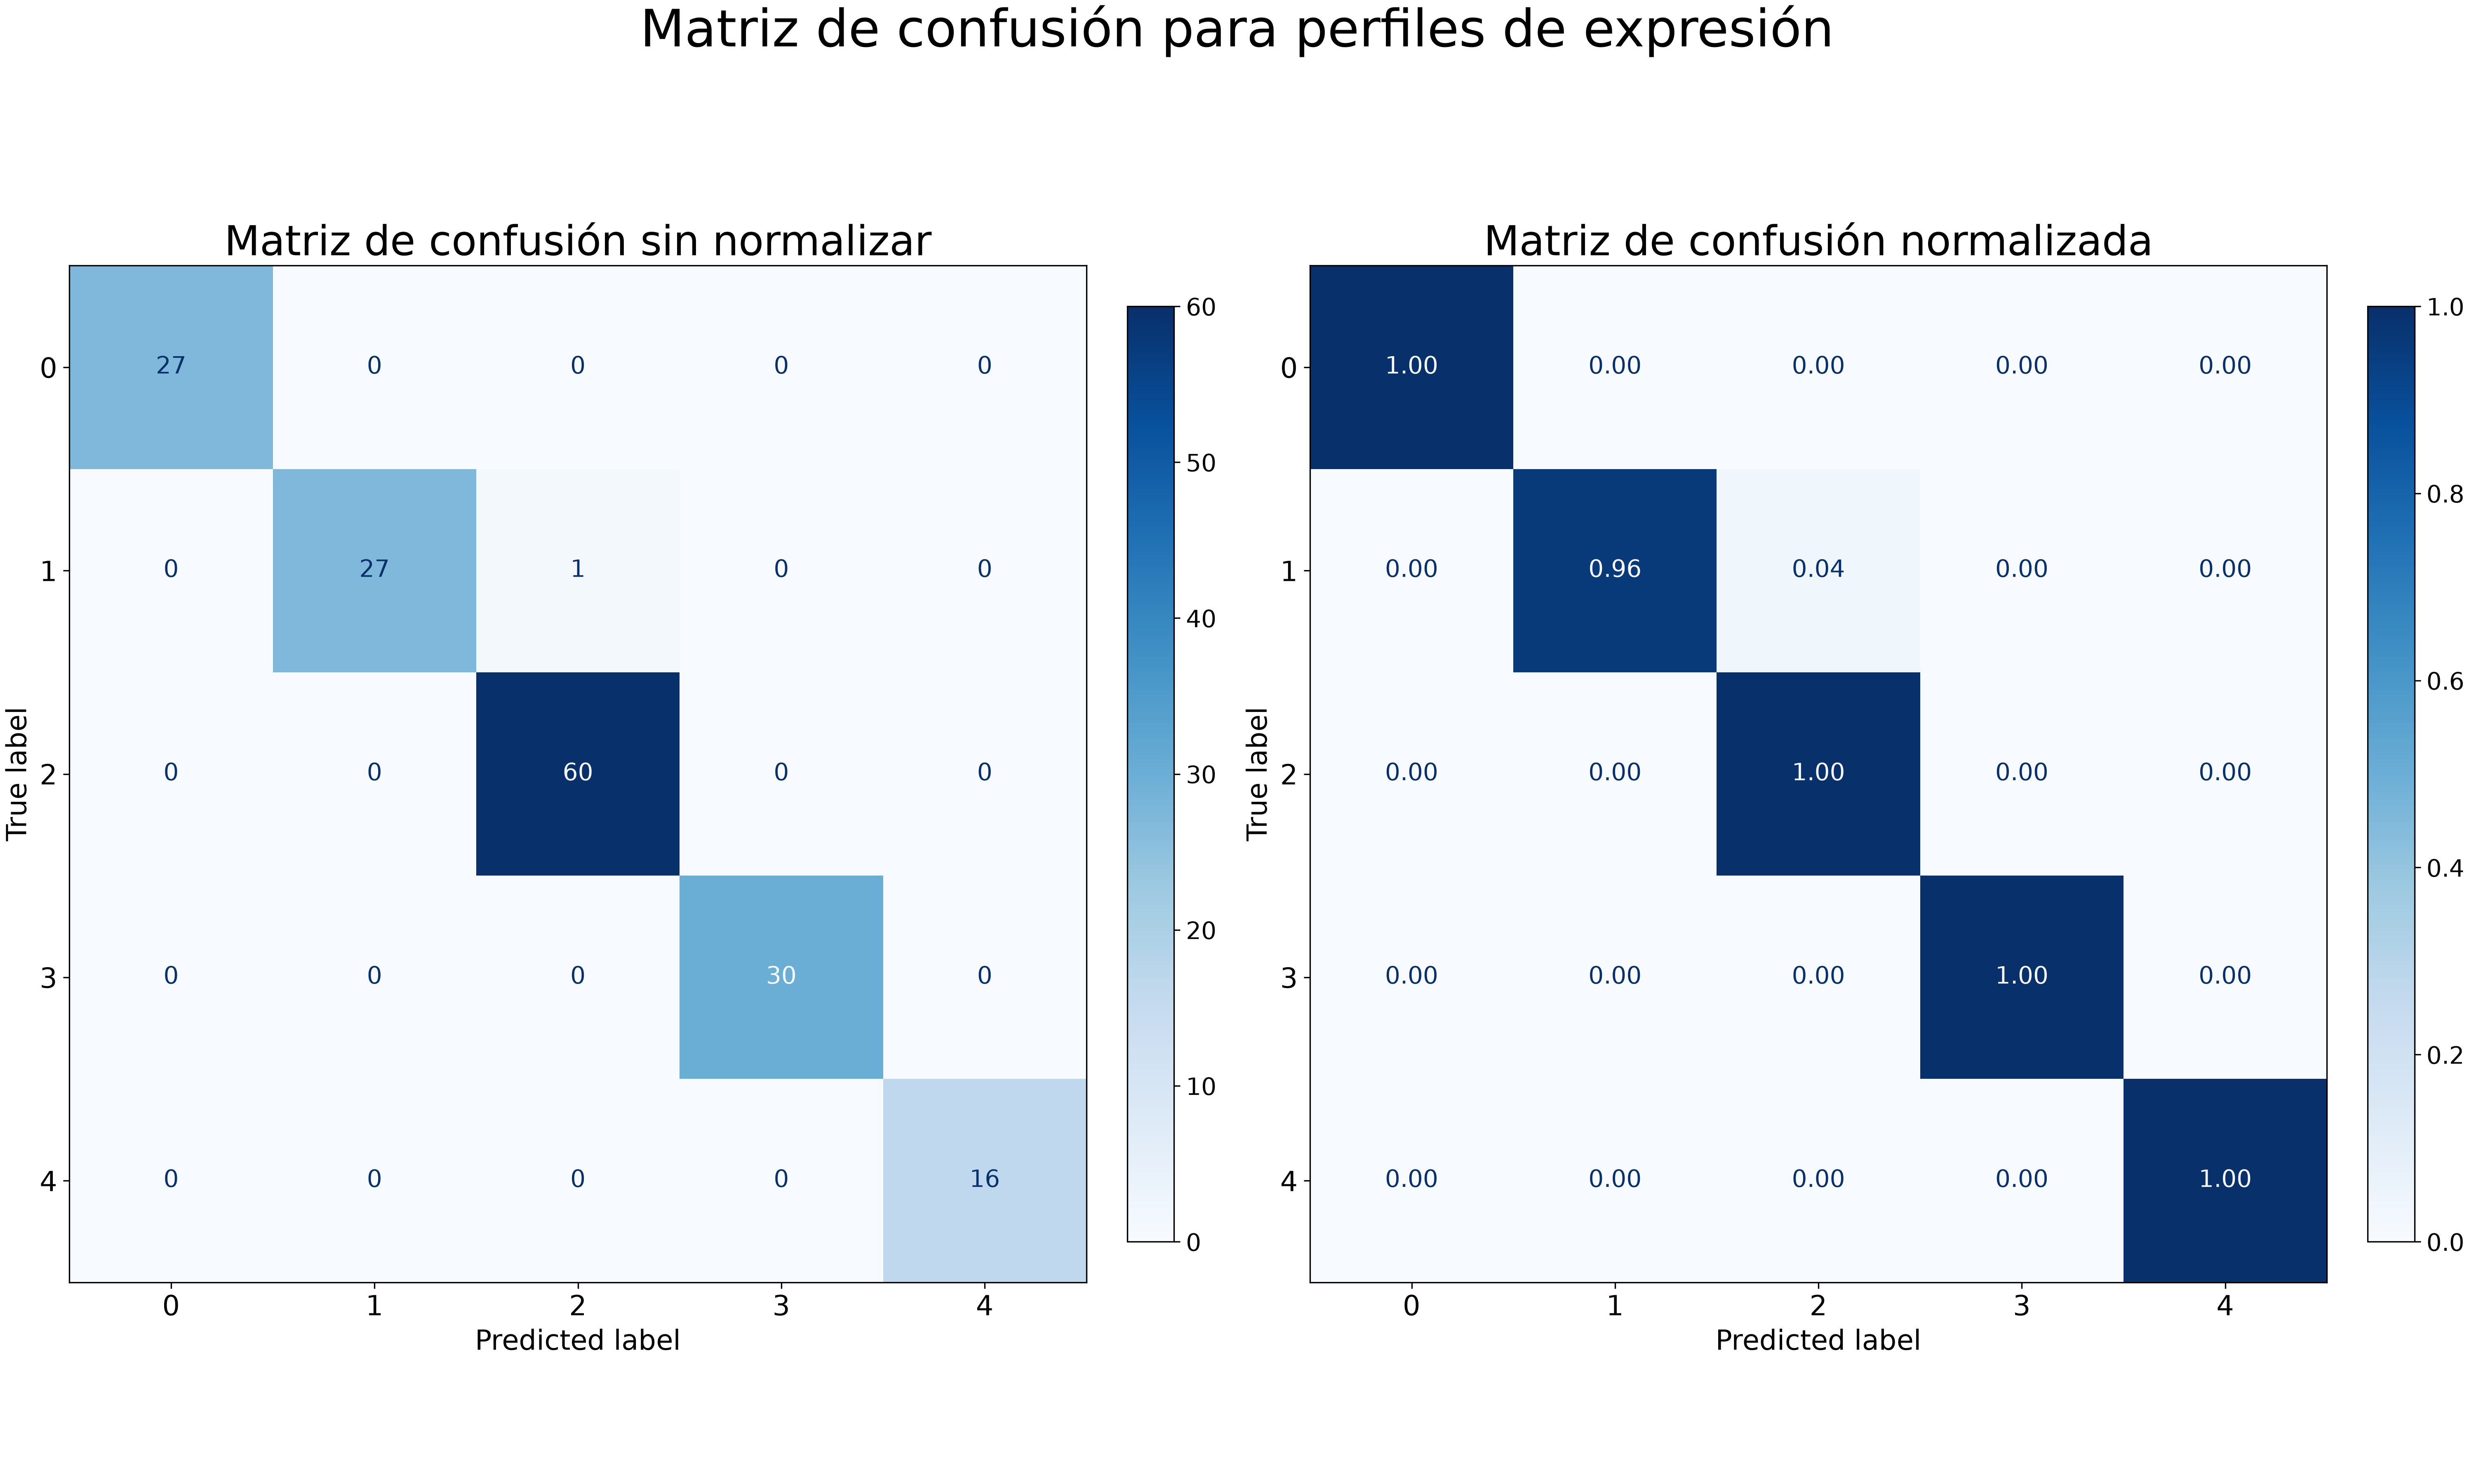
\includegraphics[width=0.85\linewidth,height=\textheight,keepaspectratio]{../res/NN/confusion_matrix_profiles_MLP.png}

}

\caption{\label{fig-aligned-vs-time}Matriz de confusión de MLP en ambos
formatos, normalizada y absoluta}

\end{figure}%

La matriz de confusión exiende de forma comprobatoria las asumciones de
las metricas antes presentadas, ya que la categoria numero 1 esta siendo
confundida con la categoria numero 2, mientras que las otras categorias
no presentan confusión alguna. Esto sugiere que son perfiles de
expresión más similares entre ambos tipos de cancer y que los demas
cuentan con factores muy diferentes en los mismos, lo que los hacen más
distinguibles.




\end{document}
